\documentclass{article}
\usepackage[utf8]{inputenc}
\usepackage{graphicx}
\usepackage{hyperref}
\usepackage{pgfplotstable}
\usepackage{geometry}
\geometry{
 a4paper,
 left=30mm,
 right=30mm,
 top=20mm,
 bottom=20mm
}


\title{EECS 447 Course Project: Goop}
\author{Zai Erb, Nicholas Nguyen, Chinh Nguyen}
\date{}

\begin{document}

\maketitle

\tableofcontents

\newpage

\section{Introduction}

Goop is an application that allows users to view, save, share, and find songs, albums, DJ Mixes, and artists. Its primary feature is its fine-tuned searching and cataloging of music based on any user-given parameters. The database allows users to see specific information about music such as release date, record label, performing artists, DJ mixes, and more. For example, if a user wants to display every DJ mix that contains a specific song or artist–or if they want to see a record label's discography from a specified timeframe. 

Each user account with their profiles and account information are stored in the database. Additionally, users are able to save and organize their music. Users are allowed to follow each other in addition to artists, labels, genres. This service is primarily useful for DJs/performers who are "crate digging" or finding new music to play in their mixes. Being able to fine-tune search results based on adjacent information (such as which mixes a song was played in or the labels an artist is on) in a collection will assist in organizing record libraries in external applications like Rekordbox, Serato, or VirtualDJ. 

The concept for Goop was born from frustrations we have had with the existing options for music cataloging. There are lots of options but all of them have significant drawbacks, the biggest of which is that they all have a narrow scope, designed to focus on one specific aspect of music cataloging and categorization, the other issue that is ubiquitous with these sites is a severely outdated, often hard to navigate UI. Rate Your Music and Album of the Year exist for rating, reviewing, and cataloging tracks and albums but neither of them provide tracklists for DJ mixes and while Rate Your Music has more data, depth, and flexibility the UI is far worse than the simpler but cleaner Album of the Year site. For getting tracklists of DJ mixes there are a few options such as 1001Tracklists, TracklistsDB and Tracklists.net all provide similar functionality but their interfaces are outdated and the integration of the tracklists with other information such as the album tracks are from, their release dates, their associated record labels, the genre of the individual tracks etc. For finding events in your area and finding electronic music recommendations Resident Advisor is fantastic however it is limited mostly to electronic music and the mixes posted on the site do not have tracklists. All of this makes for a frustrating and tedious experience for those that want to dig for music using one platform with a database that connects Albums, Genres, Mixes, Labels, Artists, Events and more. 

The biggest challenge for creating an application like this is populating the database. A lot of the aforementioned sites rely on community contribution and/or integrate with streaming services such as spotify to ensure new music is added to the database. Seeing as implementing solutions like this would not be feasible for our timeline we relied on scraping data from some of these existing sites to test our database schema and user interface. If we were to continue with this project we would enable to user contributions and could potentially integrate with streaming services to constantly update the database with newly released music.

In this report we will detail what we cover what our app is capable of currently, our methodology including how we constructed our database and schema as well as how we built the UI. We will also cover plans to expand the functionality in the future.



\section{Project Compoonents}
    \subsection{SQL} code to create tables and views in database hosted on phpMyAdmin
    \subsection{PHP backend server} to handle interaction with the database
    \subsection{Python scripts} for webscraping:
    \begin{itemize}
        \item Scraper to collect data from resident advisor using GraphQL SQL Queries
        \item Scraper to collect tracklists from tracklist.net
        \item Script to parse json files containing genres and subgenres into our tables
    \end{itemize}
    \subsection{React App} 
    \begin{itemize}
        \item Handle front end for displaying information from the backend
        \begin{itemize}
            \item Search functionality allows user to query on any of the tables
            \item Filters:
            \item Varies by page allowing users to implement filters on the page they are on.
        \end{itemize}
        \item Genre page:
        \begin{itemize}
            \item Displays genres as clickable dropdown menus to display subgenres belonging to a genre.
        \end{itemize}
        \item Artists page:
        \begin{itemize}
            \item Displays artists according to filters set by the user: options to filter by genre, year and label.
        \end{itemize}
        \item Mixes Page:
        \begin{itemize}
            \item Displays DJ Mixes according to filters set by the user: options to filter by recommended, genre, year and label.
        \end{itemize}
        \item Albums Page:
        \begin{itemize}
            \item Displays Albums according to filters set by the user: options to filter by recommended, genre, year and label.
        \end{itemize}
        \item Current Features:
        \begin{itemize}
            \item Interactive pages built on Genres, Albums, Artists, Mixes and Labels tables.
            \item Filter and search by album, genre, artist, track, label, year and more.
        \end{itemize}
        \item Future Features:
        \begin{itemize}
            \item Users database that allows users to follow other users as well as any other category within the database.
            \item Ability for users to add entries.
            \item Integration with streaming services to regularly and automatically update the database.
            \item Tree view to more easily visualize connections.
        \end{itemize}
    \end{itemize}


\section{Requirements Analysis}

\subsection{Constraints}

\subsubsection{Entity-Relationship Constraints}
\begin{itemize}
    \item Each user must have a unique username.
    \item Each artist, genre, and label should have a unique identifier.
    \item Albums, tracks, and DJ mixes should be uniquely identified.
\end{itemize}

\subsubsection{Referential Integrity Constraints}
\begin{itemize}
    \item Ensure that foreign key constraints are in place to maintain referential integrity. For example, an album should belong to a specific artist, genre, and label.
    \item Tracks within an album should be linked to the respective album they belong to.
    \item Users can only follow existing entities in the database (users, artists, labels, and genres).
\end{itemize}

\subsubsection{Data Integrity Constraints}
\begin{itemize}
    \item Implement constraints to enforce data integrity, such as NOT NULL constraints for mandatory fields.
    \item Define constraints to ensure that publication dates are valid and reasonable.
    \item Implement check constraints to validate data against specific criteria, such as ensuring publication dates are not in the future.
\end{itemize}

\subsubsection{Performance Constraints}
\begin{itemize}
    \item Consider indexing columns frequently used in search operations to improve query performance.
    \item Optimize database schema and queries to minimize response times, especially for operations involving large datasets.
\end{itemize}

\subsubsection{Consistency Constraints}
\begin{itemize}
    \item Ensure consistency across related entities. For example, if an artist's name is updated, it should reflect consistently across albums, tracks, and DJ mixes associated with that artist.
\end{itemize}

\subsection{Operations}

\subsubsection{Create Operations}
\begin{itemize}
    \item Add new users, artists, genres, labels, albums, tracks, and DJ mixes.
    \item Establish relationships between entities (e.g., users following artists, labels, or other users).
\end{itemize}

\subsubsection{Read Operations}
\begin{itemize}
    \item Retrieve information about users, artists, genres, labels, albums, tracks, and DJ mixes.
    \item Fetch lists of albums, tracks, and DJ mixes belonging to specific artists, genres, or labels.
    \item Retrieve the followers/following lists of users and entities they follow.
\end{itemize}

\subsubsection{Update Operations}
\begin{itemize}
    \item Modify user profiles, artist information, genre details, label information, album details, track details, and DJ mix details.
    \item Update relationships, such as users following/unfollowing other users, artists, genres, or labels.
\end{itemize}

\subsubsection{Delete Operations}
\begin{itemize}
    \item Remove users, artists, genres, labels, albums, tracks, and DJ mixes from the database.
    \item Delete relationships between entities, such as users unfollowing artists, genres, or labels.
\end{itemize}

\subsubsection{Search Operations}
\begin{itemize}
    \item Search for users, artists, genres, labels, albums, tracks, and DJ mixes based on various criteria (e.g., name, genre, publication date).
    \item Perform advanced searches, such as finding tracks by artist or album name, or finding users with similar tastes.
\end{itemize}

\subsubsection{Aggregate Operations}
\begin{itemize}
    \item Calculate statistics, such as the number of users following a particular artist, label, or genre.
    \item Aggregate data, such as counting the total number of albums, tracks, or DJ mixes in the database.
\end{itemize}

\subsubsection{Transactional Operations}
\begin{itemize}
    \item Execute transactions to maintain data consistency and integrity (e.g., updating multiple entities atomically).
    \item Ensure that operations such as following/unfollowing entities are performed reliably and consistently.
\end{itemize}

\subsubsection{Reporting Operations}
\begin{itemize}
    \item Generate reports on user activity, popular artists/genres/labels, trending albums, tracks, or DJ mixes.
    \item Provide insights into user preferences and behavior based on their interactions with the platform.
\end{itemize}



\section{Conceptual Design - ER Diagrams}

\subsection{Original ER Diagram}
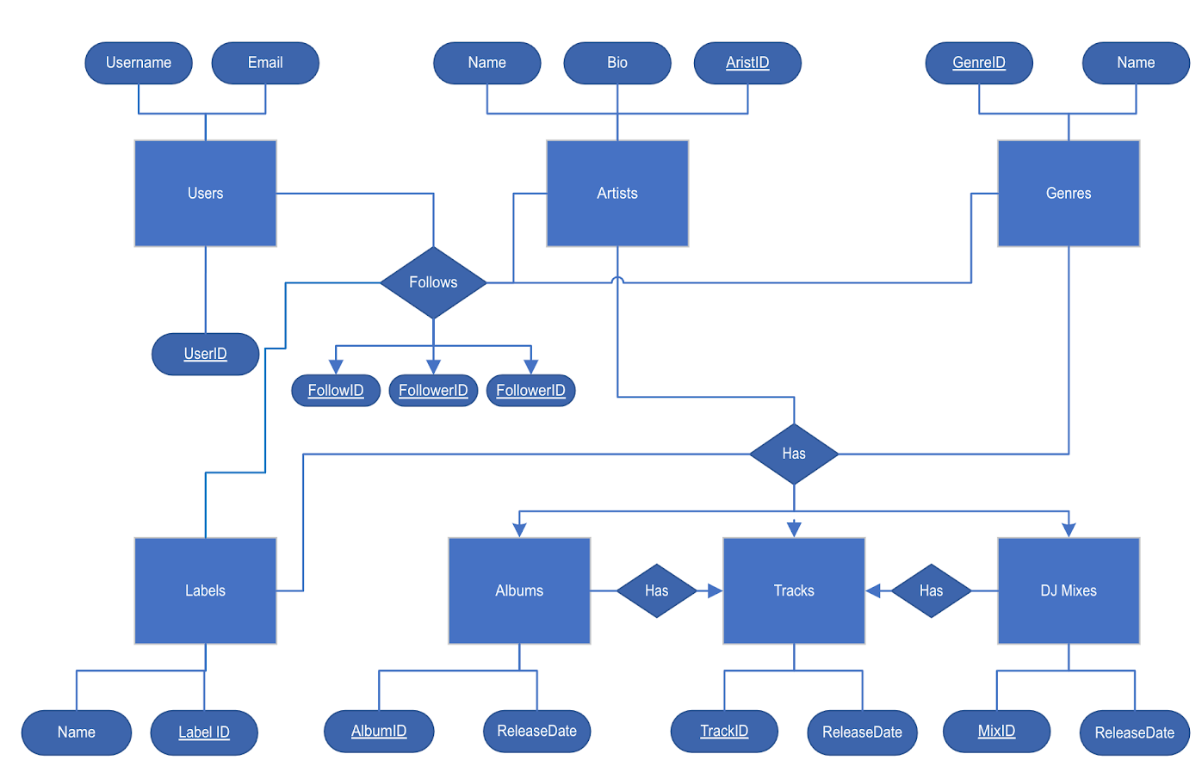
\includegraphics[width=\linewidth]{original_ER_diagram.png}

\subsection{Current ER Diagram}
\includegraphics[width=\linewidth]{path_to_current_ER_diagram.jpg}

\section{Logical Design - Relational Schemas}

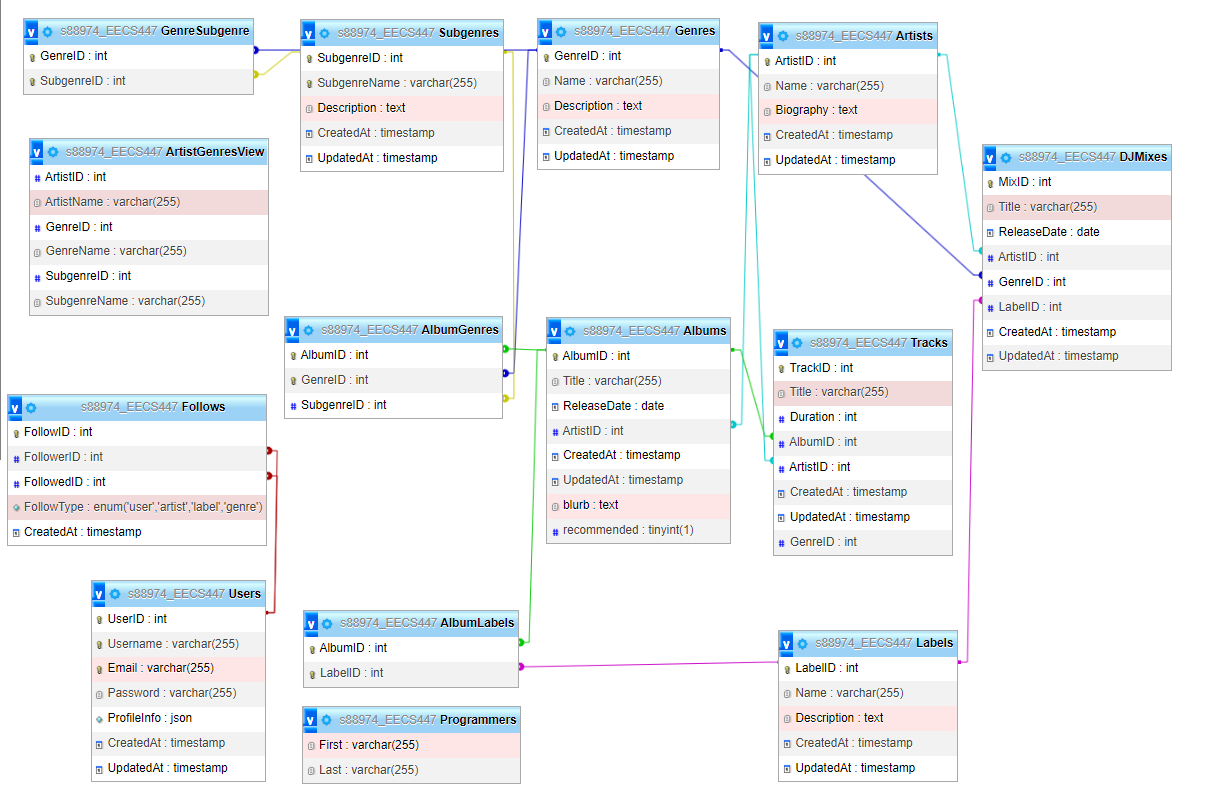
\includegraphics[width=\linewidth]{relational_schema.png}


\section{Project Log}
\begin{table}[h!]
    \centering
    \resizebox{\textwidth}{!}{%
      \begin{tabular}{|c|c|c|}
\hline
Author & Date & Message \\
\hline
Zai Erb & 2024-05-06 & Added Report and Todo List \\
Zai Erb & 2024-05-06 & Added Report and Todo List \\
Zai Erb & 2024-05-02 & Added SQL views to simplify queries \\
Zai Erb & 2024-05-02 & Improved Scraper \\
Zai Erb & 2024-04-29 & Updated Styles \\
Zai Erb & 2024-04-29 & Added resident advisor scraper \\
Zai Erb & 2024-04-18 & styling \\
Chinh Nguyen & 2024-04-18 & Navigation bar now reflects the current page when site is refreshed \\
Zai Erb & 2024-04-18 & Search Styling \\
Zai Erb & 2024-04-17 & Styling \\
Chinh Nguyen & 2024-04-17 & STYLING! \\
Chinh Nguyen & 2024-04-17 & Fixed fetching tracks by artistName, doesn't have to be exact match now \\
Zai Erb & 2024-04-17 & Styling \\
Chinh Nguyen & 2024-04-17 & Cleaned up CSS, made scrollable, fixed naming \\
Chinh Nguyen & 2024-04-17 & Added search for tracks by artist name \\
Chinh Nguyen & 2024-04-17 & Added fetching tracks by artist name \\
Zai Erb & 2024-04-17 & Updated styling \\
Zai Erb & 2024-04-17 & Added GenreClick functionality for all pages. \\
Zai Erb & 2024-04-17 & Added all pages to sort items by Genre \\
Chinh Nguyen & 2024-04-17 & Implemented search artists by genreID \\
Chinh Nguyen & 2024-04-17 & Added 5th query with JOIN: Get artists based off GenreID \\
Chinh Nguyen & 2024-04-17 & Results Textarea \\
Zai Erb & 2024-04-17 & Genre Components \\
Chinh Nguyen & 2024-04-17 & Updated to include Search page \\
Chinh Nguyen & 2024-04-17 & Two new queries: Search Tracks based off genreID and title \\
Chinh Nguyen & 2024-04-17 & Basic Search Page \\
Zai Erb & 2024-04-17 & Added 1001 scraper. Not working \\
Chinh Nguyen & 2024-04-17 & Added more function \\
Chinh Nguyen & 2024-04-17 & Added Subgenre fetching using INNERJOIN on GenreID and SubgenreID \\
Chinh Nguyen & 2024-04-17 & Subgenre Fetch Function + Dropdown Divs \\
Chinh Nguyen & 2024-04-17 & Added query for Subgenre table: SubgenreName and Description \\
Chinh Nguyen & 2024-04-17 & Oops. Fixed reading of config.json \\
Nicholas Nguyen & 2024-04-17 & Fixed Genre alignment (along with other elements)

fixed weird redundancies too shared between each file.

added heart easter egg too because why not \\
Chinh Nguyen & 2024-04-17 & Necessary Packages Required, Added Localhost with Port 3001 as Proxy (IMPORTANT FOR BACKEND) \\
Chinh Nguyen & 2024-04-17 & Connected to the backend and displays "Genres" table with "Name" and "Description" column \\
Chinh Nguyen & 2024-04-17 & Working starter backend -- run with "node akiserver.js" in a second terminal, make sure that no other program is running port 3001 \\
Chinh Nguyen & 2024-04-17 & Password Leak -- Rotated Password / See Discord \\
Zai Erb & 2024-04-16 & Updated Genres Page - functional for presentation \\
Zai Erb & 2024-04-16 & Updated components and genre jsons \\
Zai Erb & 2024-04-16 & Updated JSON format \\
Zai Erb & 2024-04-16 & Fixed gitignore merge conflict \\
Zai Erb & 2024-04-16 & data changes \\
Zai Erb & 2024-04-16 & Data Changes \\
Nicholas Nguyen & 2024-04-16 & Furthered Front-End Design/Development \\
Nicholas Nguyen & 2024-04-15 & Add files via upload \\
Zai Erb & 2024-04-15 & Updated Scraper \\
Nicholas Nguyen & 2024-04-15 & Create .gitignore \\
Zai Erb & 2024-04-15 & Added raw data for genres in JSON files and added script to convert JSON into SQL tables \\
Zai Erb & 2024-04-03 & Added react project files \\
Zai Erb & 2024-04-03 & first commit \\
\hline
\end{tabular}
    }
  \end{table}


\end{document}
